\section{实验结果分析}
MNIST数据集通过torchvision加载,所有算法基于python的numpy实现,数据预处理的一部分地方借助pytorch实现. 细节请参考:\\
\url{https://github.com/WANGH950/Statistical-Machine-Learning/tree/main/1ST }

\subsection{感知机学习算法结果分析}

\begin{figure}[htpb]
    \centering
    \subfigure[感知机原型算法训练结果]{
		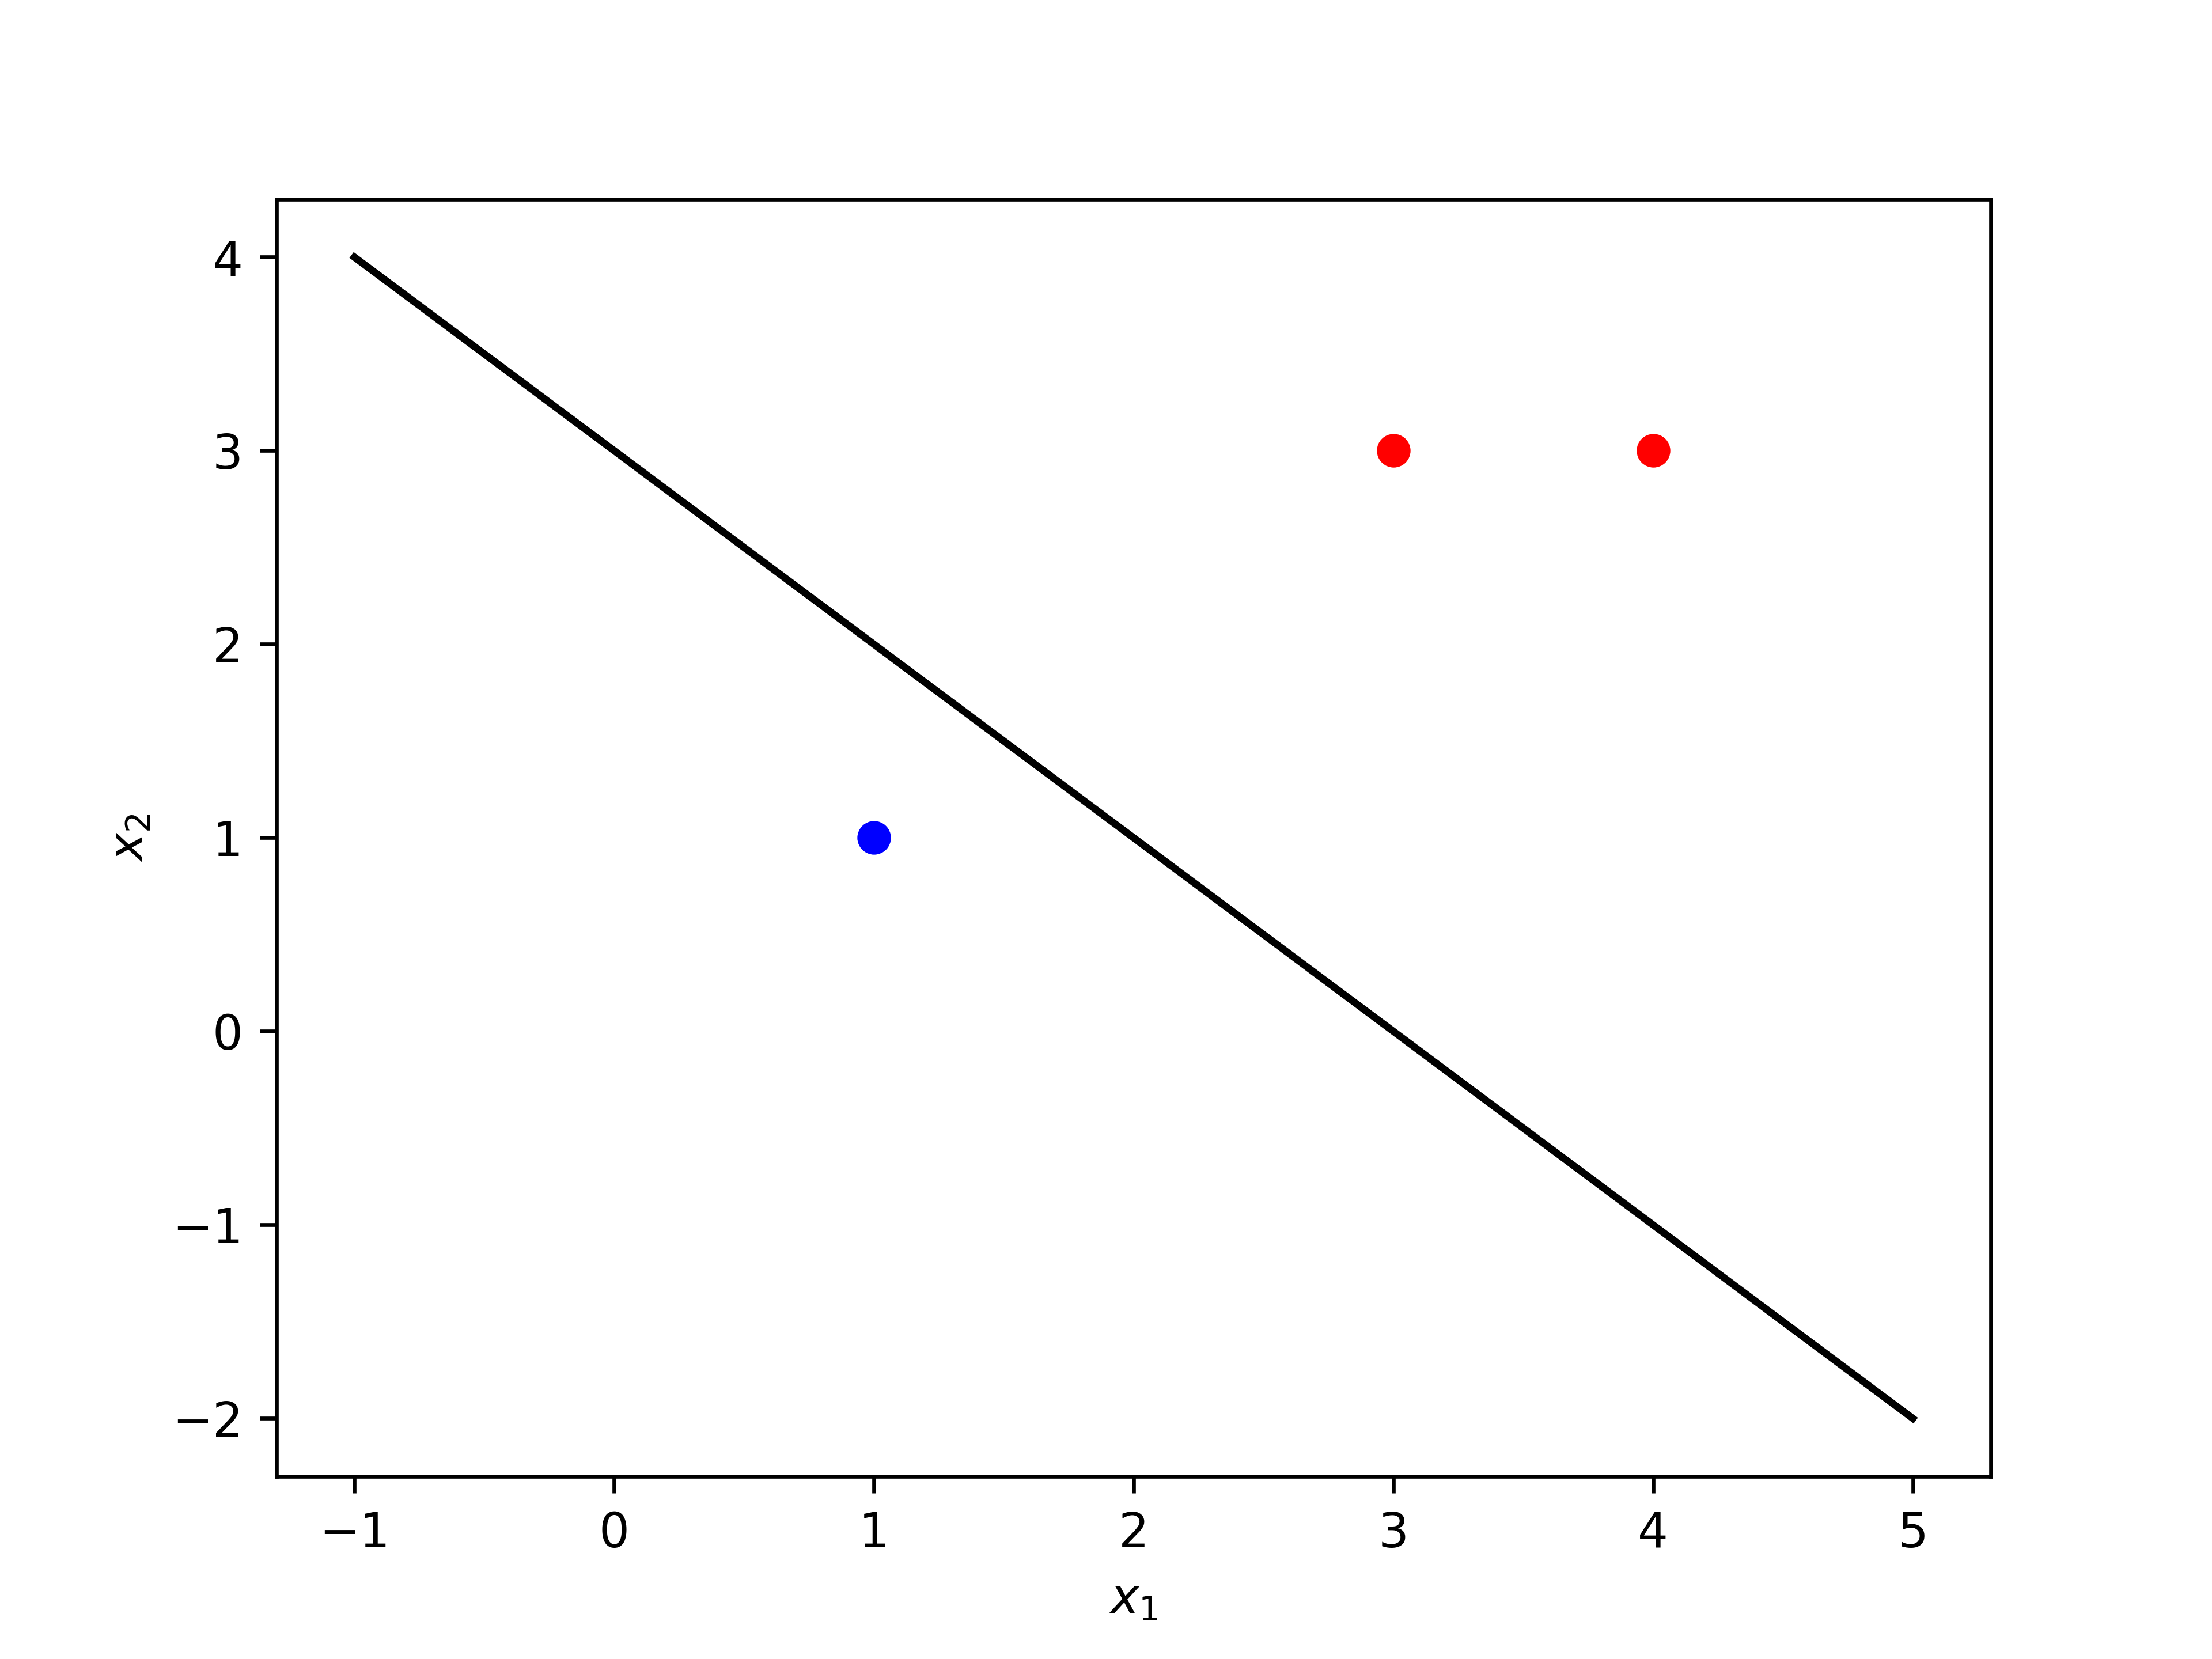
\includegraphics[width=0.48\linewidth]{figure/perception1.png}}
	\subfigure[感知机对偶算法训练结果]{
		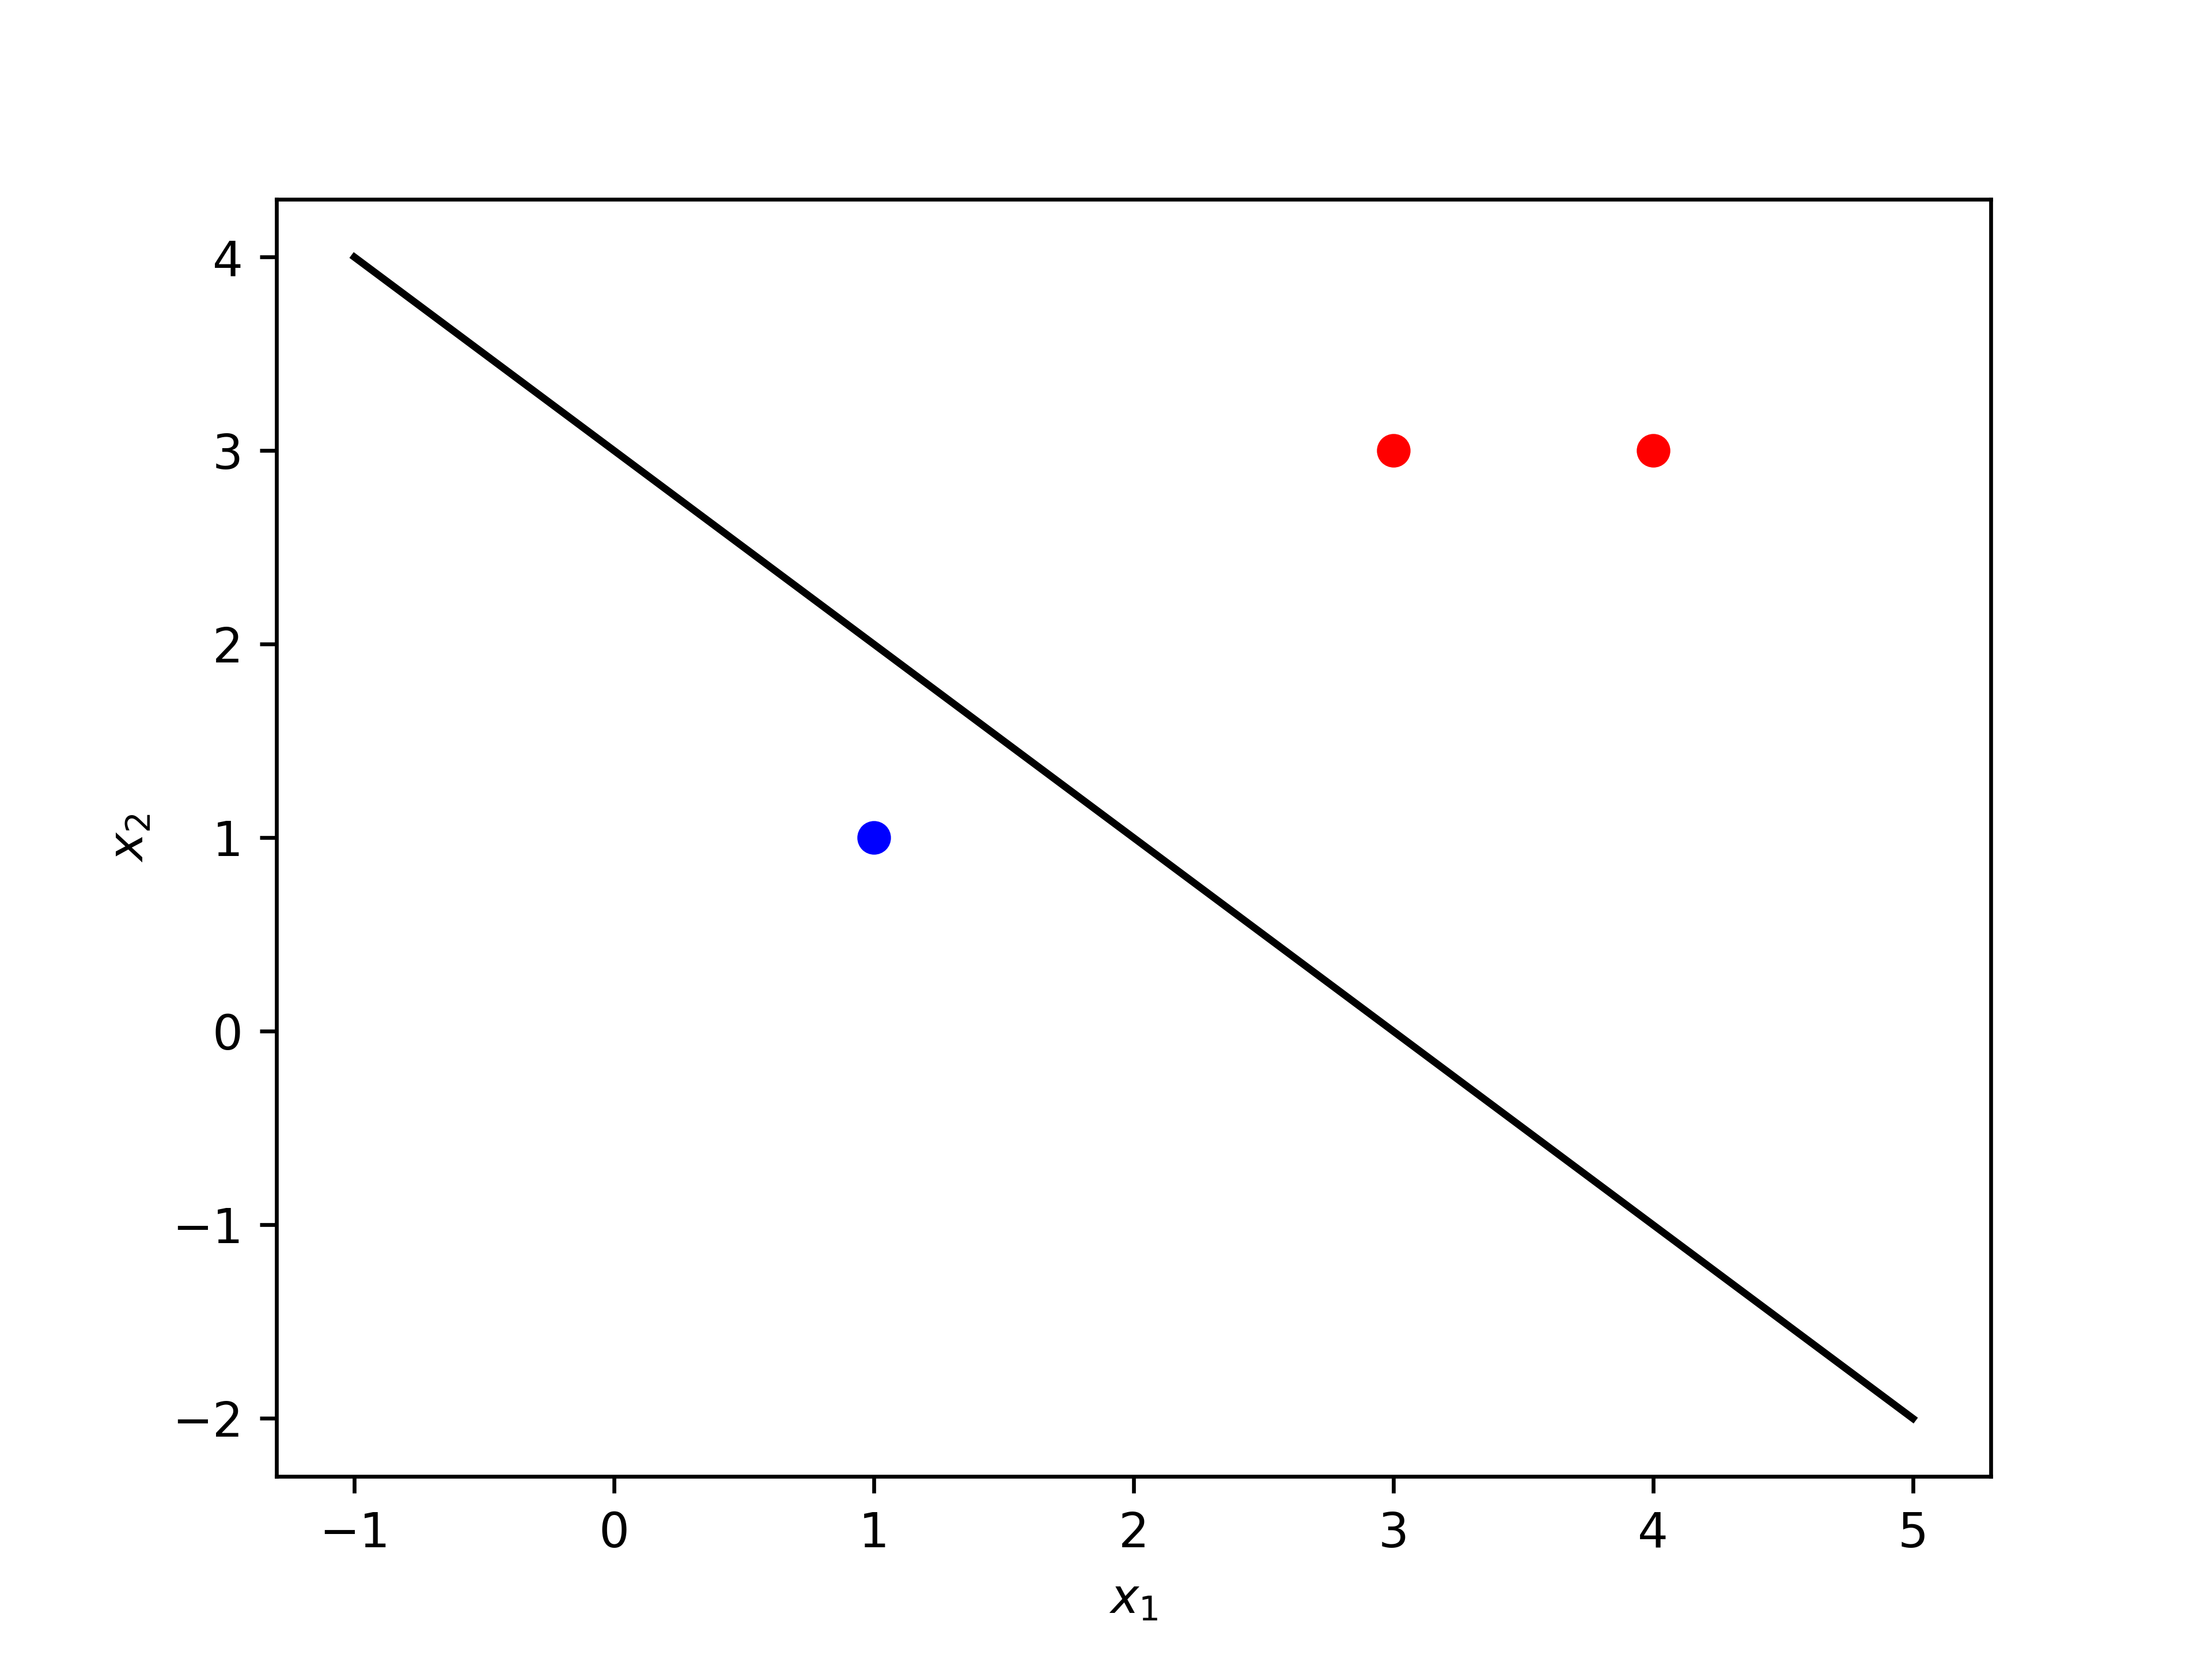
\includegraphics[width=0.48\linewidth]{figure/perception2.png}}
    \caption{感知机模型训练结果, 其中红点表示正类, 蓝点表示负类, 黑色实线表示感知机分割超平面.}
    \label{figure2}
\end{figure}

以$0.01$的学习率, 感知机原型算法在题目给定的数据上, 经过$5$次训练后收敛, 得到结果.
以$0.01$的学习率, 感知机对偶算法在题目给定的数据上, 经过$5$次训练后收敛, 得到结果. (图 \ref{figure2})

\begin{lstlisting}[caption = MNIST数据加载]
import torchvision
data=torchvision.datasets.MNIST(
    root='MNIST',
    train=True,
    transform=torchvision.transforms.ToTensor(),
    download=True
)
\end{lstlisting}
\begin{lstlisting}[caption = MNIST数据预处理]
train_data = data.train_data
train_label = data.train_labels
# 转化为二分类
data_set = []
for i in range(train_data.shape[0]):
    if train_label[i] < 5:
        y = 1
    else:
        y = -1
    data_set.append(
        (train_data[i].reshape([28**2]).numpy()/255,y)
    )
\end{lstlisting}
\begin{lstlisting}[caption = 使用对偶感知机算法处理MNIST数据]
model = PerceptionDual(data_set[:1000])
model.train(
    epoch=30,
    learning_rate=0.001
)
\end{lstlisting}

如Listing 6所示, 我们使用$1,000$条数据, 在$0.001$的学习率下训练了$30$次, 最后在训练数据上得到了$0.923$的准确率.
\subsection{k-近邻算法结果分析}
\begin{lstlisting}[caption = MNIST数据预处理]
data_num,dimx,dimy = train_data.shape
data = train_data.reshape([data_num,dimx*dimy])+torch.randint(0,10,[data_num,dimx*dimy])
label = train_label.unsqueeze(-1)
\end{lstlisting}

如Listing 7所示, 由于手写数字是稀疏矩阵, 我们通过对其添加随机噪声以保证构造的kd-树是好的(不加噪声会导致数据都分布在一个节点上). 
这里, 我们添加$U(0,10)$的均匀整数噪声.
\begin{lstlisting}[caption = 构造kd-树]
model = KDTree()
tree = model.create(
    data=data[:30000],
    label=label[:30000]
)
\end{lstlisting}

如Listing 8所示, 我们使用前$30,000$条数据构造kd-树. 我们选取第$40,000$条数据进行预测, 图1展示了预测结果和真实结果.
\begin{figure}[htpb]
    \centering
    \subfigure[真实值]{
		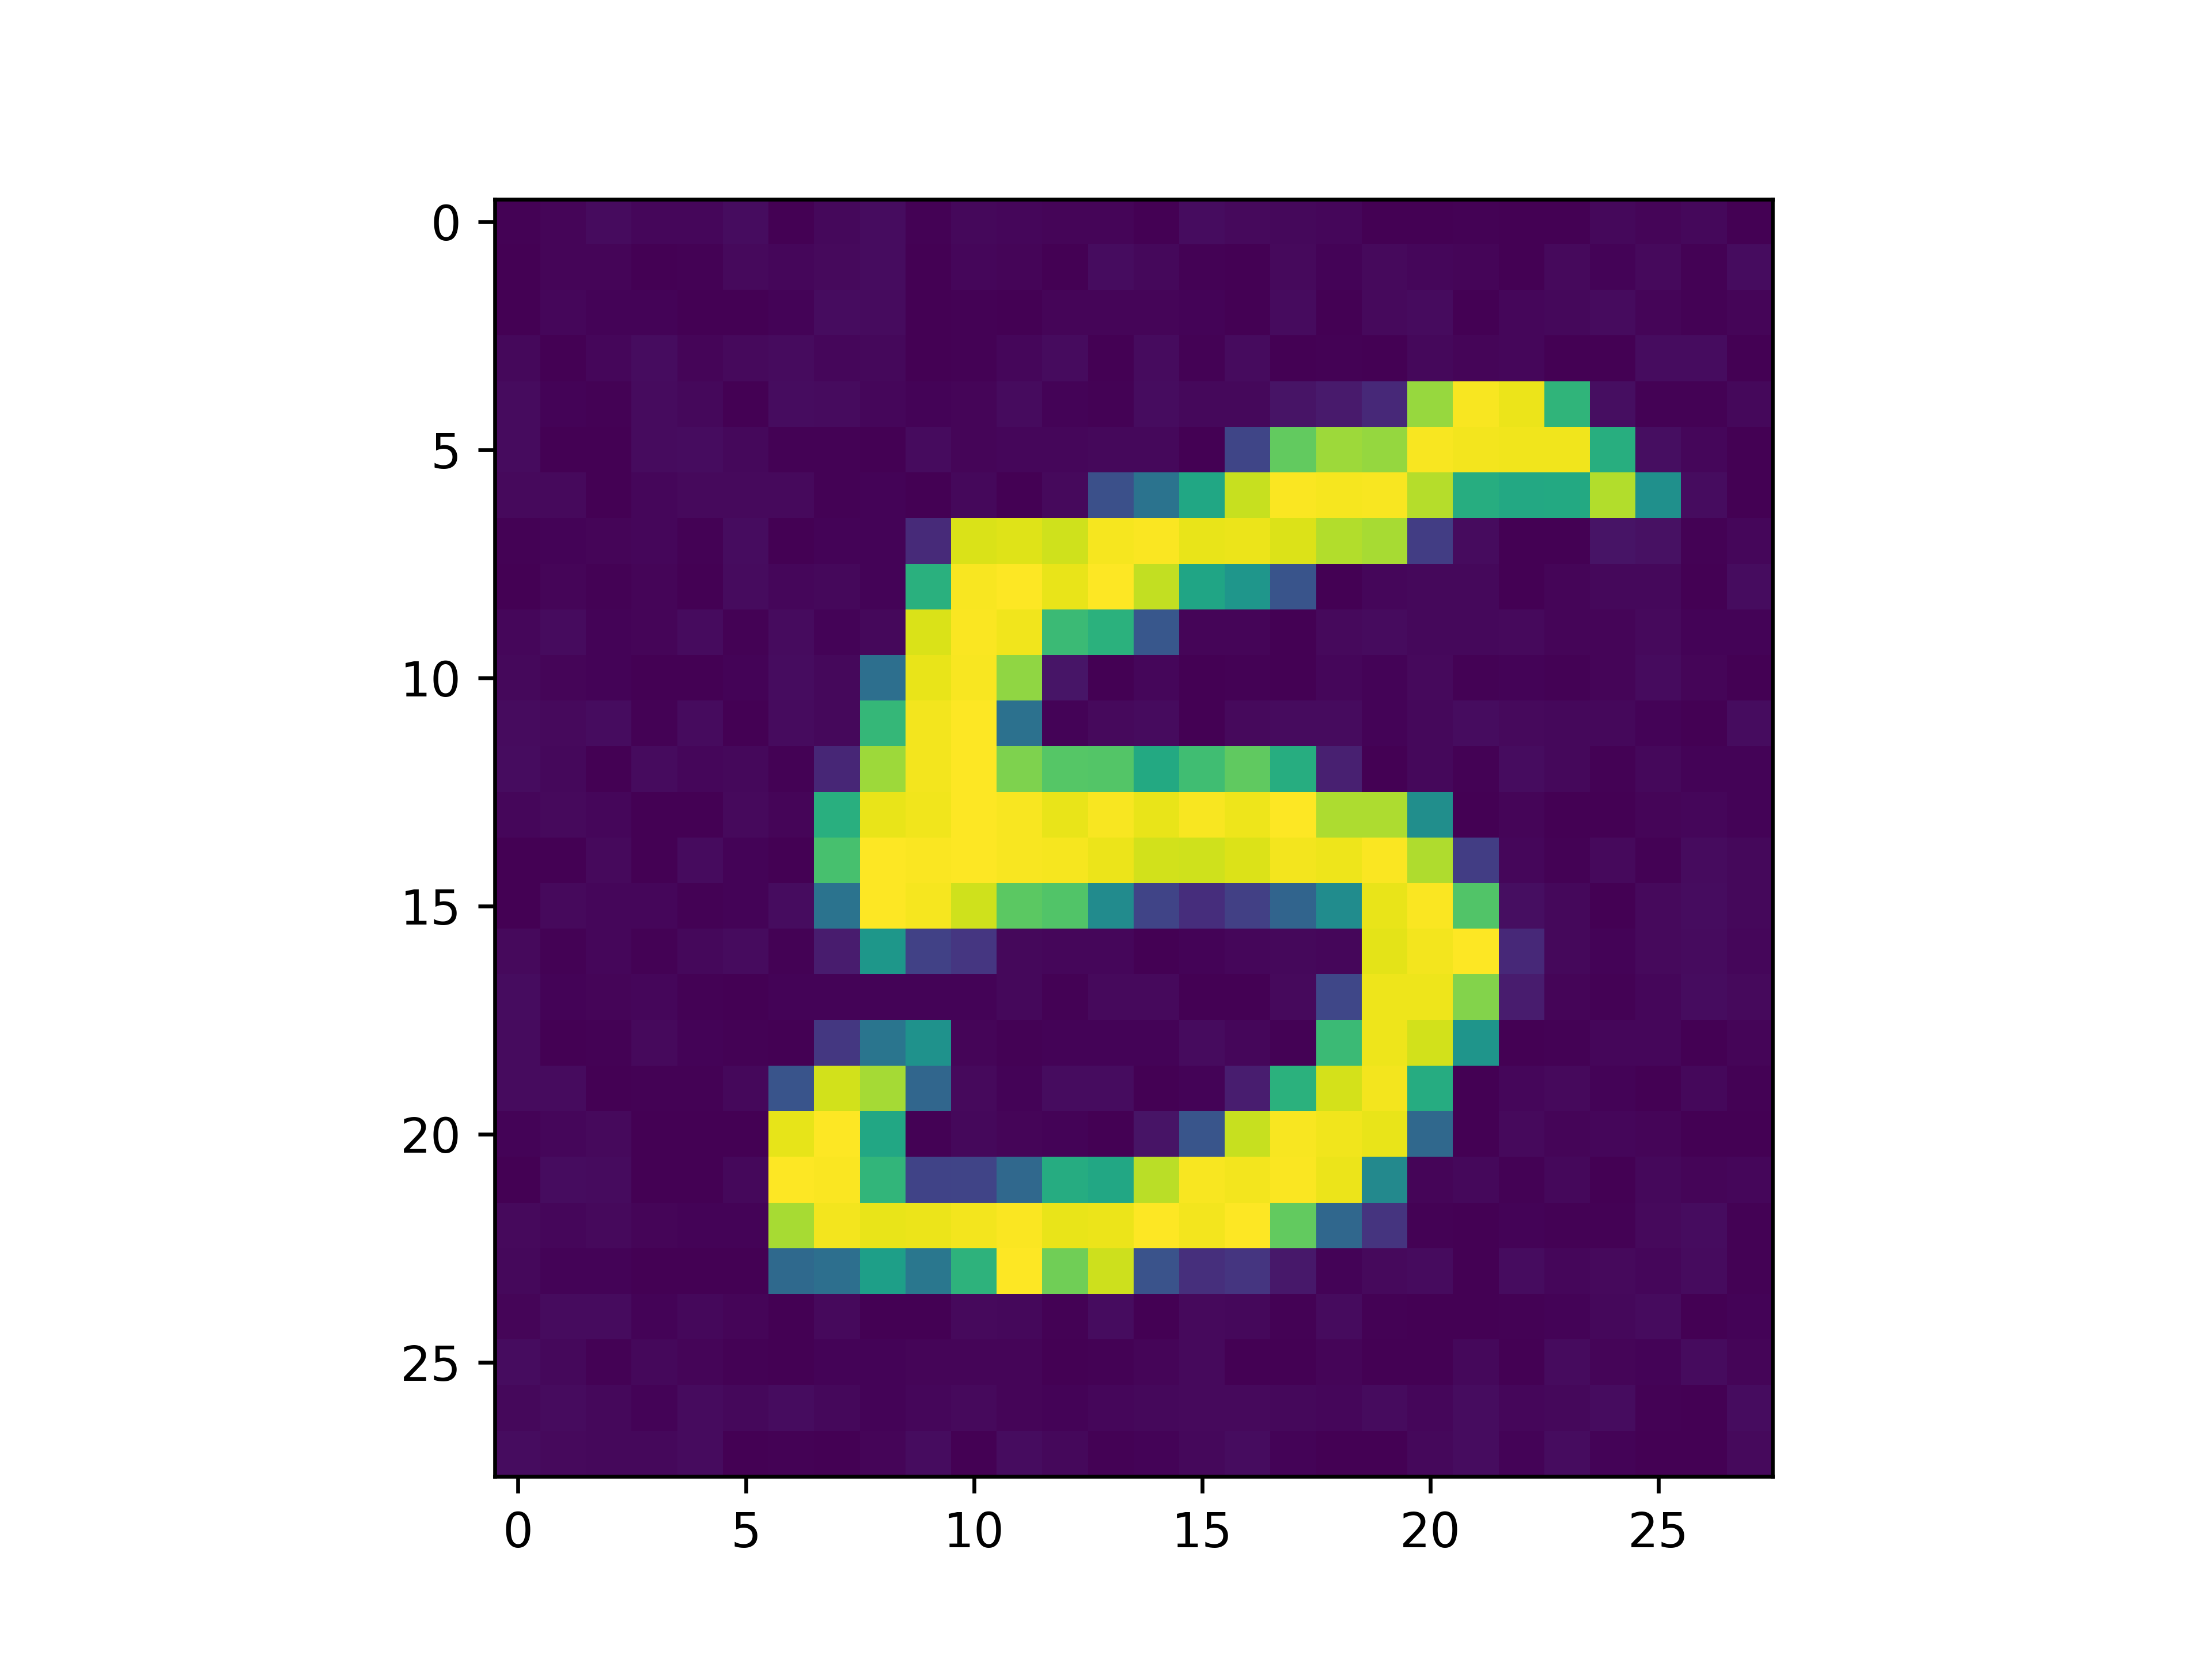
\includegraphics[width=0.48\linewidth]{figure/mnist_rel.png}}
	\subfigure[搜索得到的最近值]{
		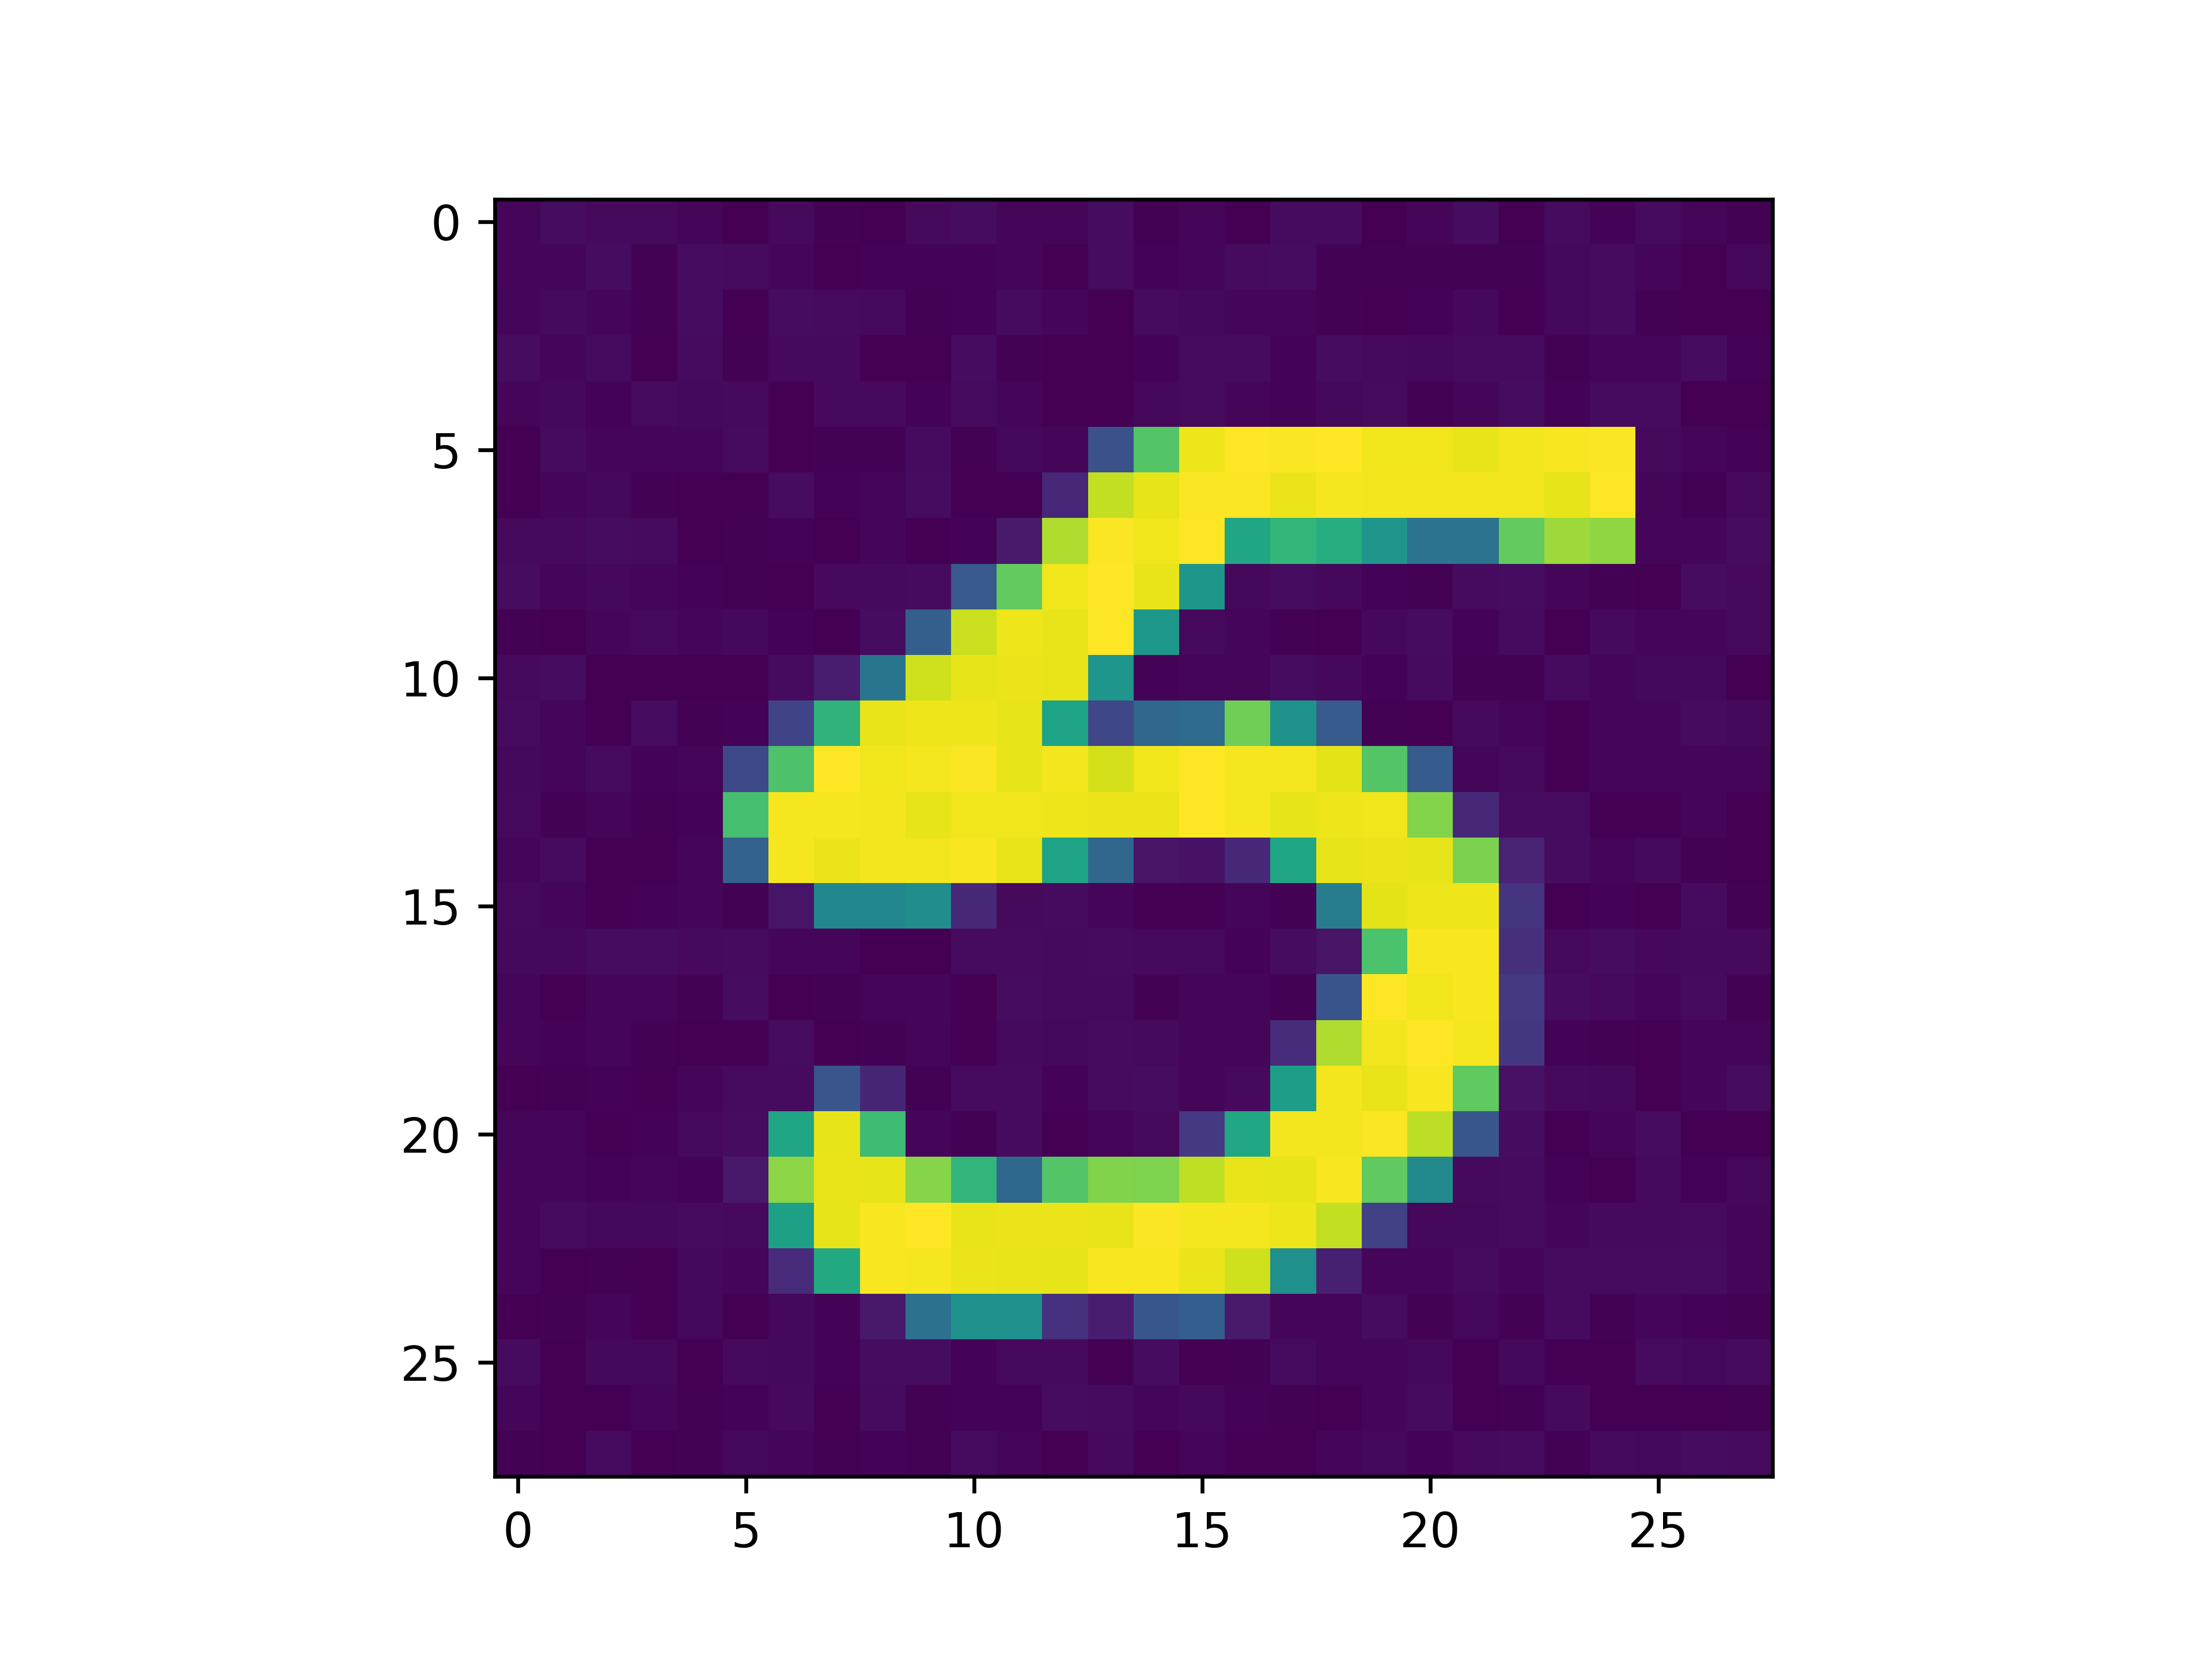
\includegraphics[width=0.48\linewidth]{figure/mnist_pre.png}}
    \caption{kd-树搜索结果.}
    \label{figure1}
\end{figure}

同时, 我们还使用后$30,000$条数据作为测试集进行测试(listing 9), 得到了$90.38\%$的准确率. 结果表明, 我们的算法实现准确.
\begin{lstlisting}[caption = 使用kd-树分类测试数据]
k = 30000
acc = 0
data_test = data[-k:]
label_test = label[-k:]
for i in range(k):
    data_rel = data_test[i]
    label_rel = label_test[i]
    data_pre,label_pre = model.search(data_rel)
    if label_pre == label_rel:
        acc += 1
acc /= k
\end{lstlisting}

所有实验结果和运行效率以源码为准: \\
\url{https://github.com/WANGH950/Statistical-Machine-Learning/tree/main/1ST }